
\begin{figure*}[t]
    \centering
    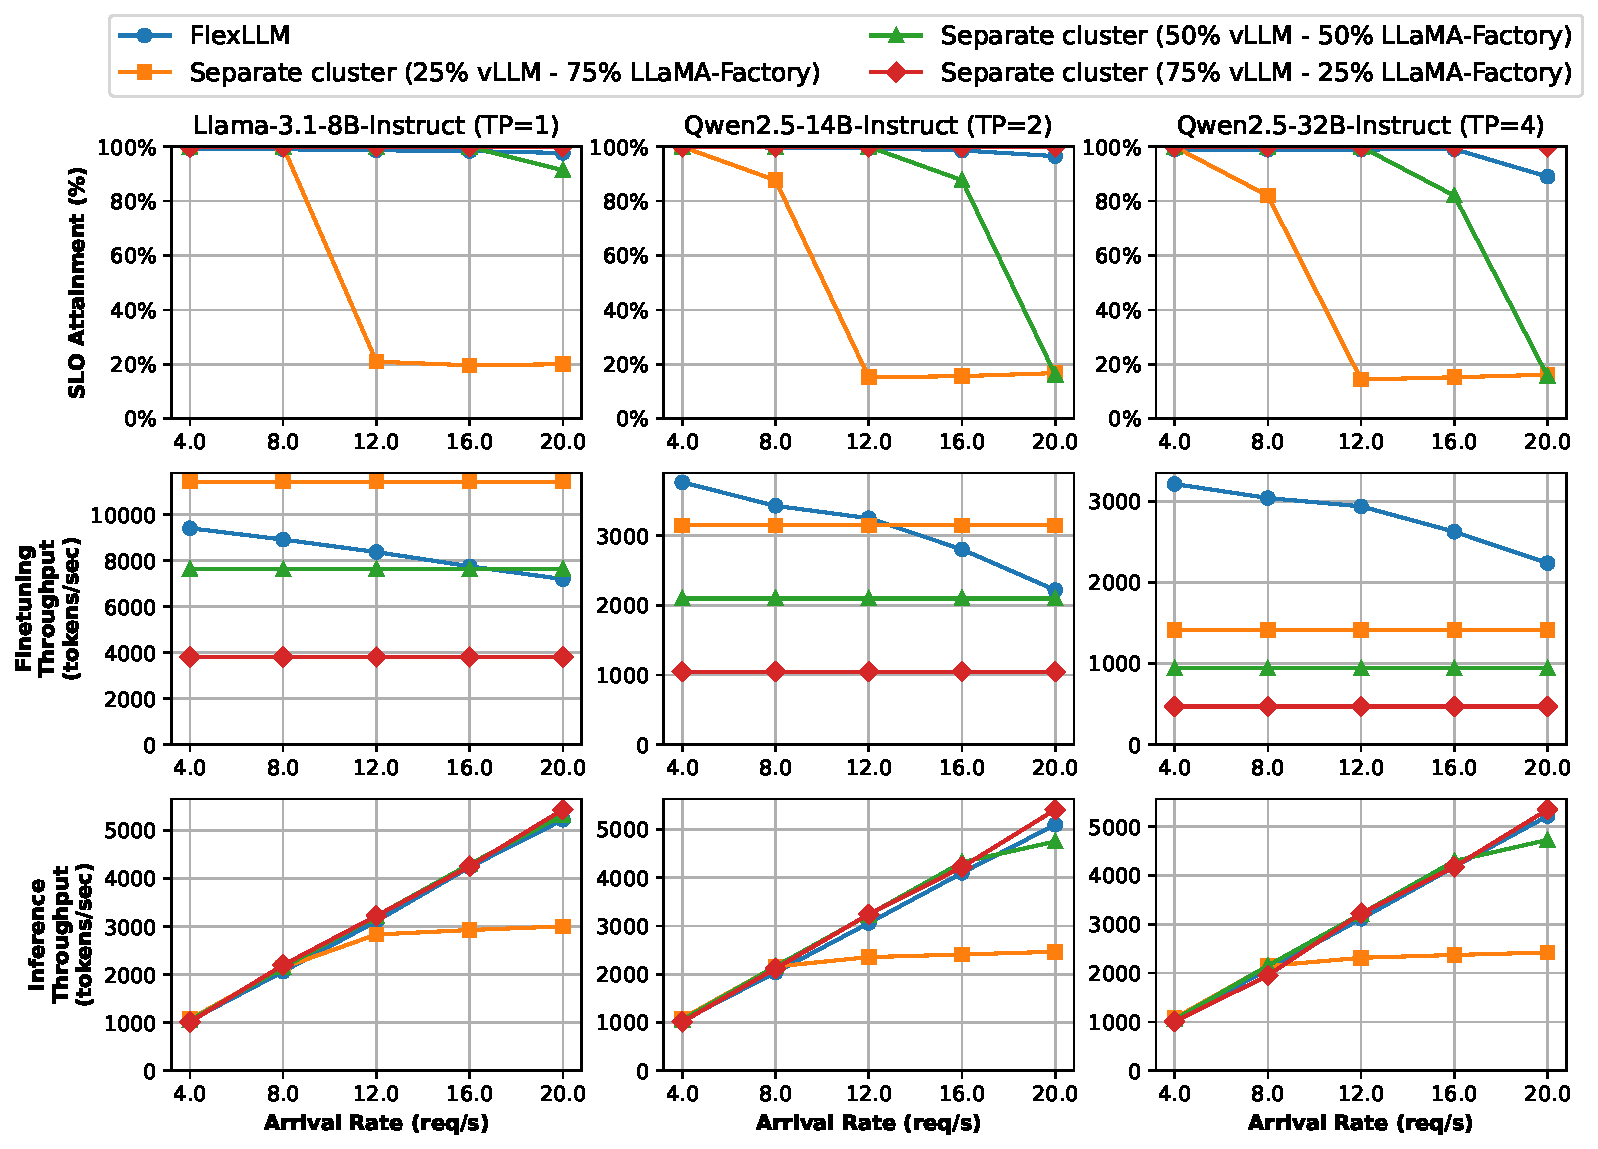
\includegraphics[width=0.75\textwidth]{figs/combined_plot.pdf}
    \caption{End-to-end comparison between co-serving and using separate resources on three models.}
    \label{fig:end-to-end}
\end{figure*}

\begin{figure*}[t]
    \centering
    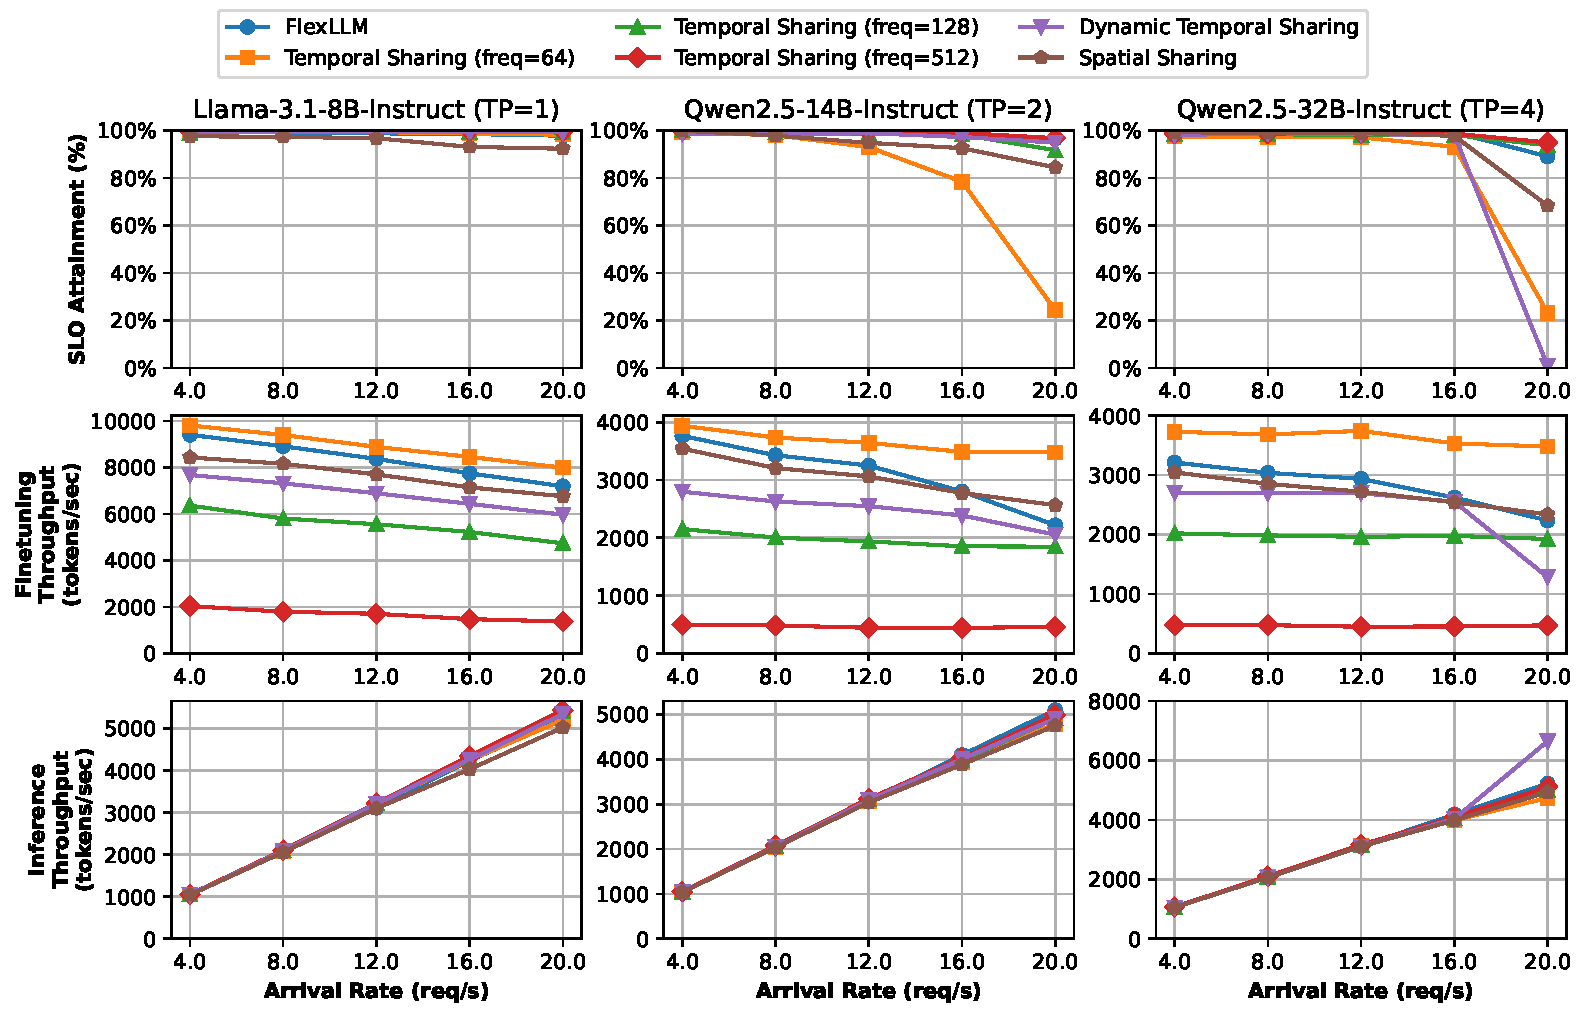
\includegraphics[width=0.75\textwidth]{figs/internal_baselines.pdf}
    \caption{End-to-end comparison of co-serving with temporal and spatial sharing strategies.}
    \label{fig:temporal-spatial-sharing}
\end{figure*}

\section{Implementation}
\label{sec:impl}
\sys is built on FlexFlow Serve~\cite{miao2023specinfer} with 9K lines of C++ and CUDA code. It provides C++ and Python bindings, with full HuggingFace compatibility for \texttt{PEFT}~\cite{peft} and \texttt{transformers}~\cite{transformers} libraries. \Sys supports PEFT models with LLAMA~\cite{touvron2023llama}, GPT~\cite{brown2020language}, OPT~\cite{zhang2022opt}, Falcon~\cite{falcon40b}, or MPT~\cite{MosaicML2023Introducing} backbones, among others. 

\paragraph{Memory management.}
\Sys manages the required GPU memory using a combination of static and dynamic allocation. Static allocation reserves GPU space for the backbone weights and the KV cache required for incremental decoding during inference. Dynamic allocation is used for gradients, activations, and optimizer states. When a finetuning request is received, \Sys allocates memory during the first forward pass and reuses it during subsequent backward passes, freeing up space when it's no longer needed.
For inference memory management, FlexLLM employs paged attention~\cite{10.1145/3600006.3613165} with chunked prefill~\cite{agrawal2023sarathi} to dynamically allocate KV cache pages and minimize evictions. New inference requests are only admitted if the entire prompt can fit within available KV cache pages, preventing memory fragmentation and ensuring stable inference performance during co-serving.

\paragraph{Key-value gradient accumulator.}
To support token-level finetuning, it is necessary to accumulate key-value gradients for every preceding token in a given sequence during backpropagation. \sys utilizes static allocation to reserve space for key-value gradient accumulation. During backpropagation, the gradients for keys and values of a specific segment are obtained, and the position of this segment in the overall sequence is determined. \sys then accumulates the new key-value gradients of all subsequently scheduled segments. When a segment is scheduled during backpropagation, it includes accumulated gradients from future tokens.
